\section{Chameleon OpenStack}
\label{chameleon-openstack}
\index{Chameleon!Openstack}

OpenStack on Chameleon delivers KVM based compute resources to
provision virtual machines. It provides various image types on
which we can deploy tools and software needed for the class and
projects. We will you through the basic steps of getting access to
OpenStack Chameleon cloud under the class allocation. Next, we will
introduce you to the command line tools which you can use in your
projects. Naturally using the GUI for your projects is not sufficient
as setting up your environment will need steps to be executed by hand
which is not sufficient. It is a goal of this class that you create
your environment ins a reproducible fashion via scripts.  Hence,
although the Web interface called OpenStack Horizon is initially
attractive, we should make sure to move on to the commandline
interfaces.  Furthermore, it is often difficult to resolve technical
issues as the command line tools generate full debugging messages in
case of issues and copy and past into helo windows is much easier and
efficient than copy and past incomplete screenshots.


\subsection{Outages}

Any computer system may undergo maintenance. Before filing tickets
with Chameleon cloud, make sure that the cloud is operational. Outages
are posted at 

\url{https://www.chameleoncloud.org/user/outages/}

To be notified by mail, you can subscribe to them at 

\url{https://www.chameleoncloud.org/user/profile/subscriptions/}

\subsection{Account Creation}

The fist step to get access Chameleon cloud is to create a user
account if you do not already have one. You can skip to the next
section if you have a chameleon cloud account.

The register web page is available at:

\url{https://www.chameleoncloud.org/user/register/}

For more details, please als consult the chameleon chapter in the
handbook.

\subsection{Join a Project}

An active project is required to access compute resources.  Each class
has a particular project number that you will need to write down as
you will use it to interact with the system. The information is
given out by the instructor. 

For the Spring-18 classes including i524, e516, and e616 please use
the following project number:

\begin{lstlisting}
CH-819337
\end{lstlisting}

However, before you can access it the instructor (in our class Dr. von
Laszewski) needs to authorize you to use the project. For this you
have filled out an account survey in piazza. The most common errors we
see are that students provide us with the wrong user name or have not
applied for a chameleon account. Once the instructor has added you,
you will be able to use VM's on Chameleon cloud. 

\subsection{Usage Restriction}

As using VM's in a shared environment cost resources, you are
{\underline\bf REQUIRED} to shut down your resources after you are not
using them anymore. Furthermore, before the class is over and we
assign grades you must terminate your instances and free all ip
addresses. Remember that any running VM is just like you were running
a real computer. I am sure you close the lid of your laptop when not
in use. Shutting down the VM is similar and avoids that you
unnecessarily use resources that others could use in a shared
environment.


\subsection{OpenStack RC File}

We will use the Nova command line tools for Chameleon OpenStack and to
authorize our account on the command line tools. To do so, you will
need an openstack RC file. 


\subsubsection{Creating OpenStack RC via the editor}

The easiest way is to create this file by hand while copying the
following lines into the file
\verb|~/.cloudmesh/chameleon/cc-openrc.sh|. Make sure that you place
the file in a location you easily be found:

\begin{lstlisting}
mkdir -p ~/.cloudmesh/chameleon
\end{lstlisting}

The easiest way is to download a template from pur book with 

\begin{lstlisting}
https://raw.githubusercontent.com/cloudmesh/book/master/examples/chameleon/cc-openrc.sh
\end{lstlisting}

The cc-openrc.sh looks as follows:

\lstinputlisting[language=bash]{examples/chameleon/cc-openrc.sh}

Please make sur to replace
\verb|<put your chameleon cloud username here>| with your
chameleon cloud username. Now whenever you need top access chameleon
cloud you can use the command

\begin{lstlisting}
source ~/.cloudmesh/chameleon/cc-openrc.sh
\end{lstlisting}

To simplify the configuration and documentation, we have included two
shell environment variables. The first one is \verb|CC_PROJECT|, that
specifies the project number. The second one is a prefix that you will
use for VMS and keys as we are using a shared project. This way we can
see which VMS and which keys have been uploaded and keep the names of
them unique.

\begin{lstlisting}
export CC_PROJECT=CH-819337
export CC_PREFIX=albert-111
\end{lstlisting}

\subsubsection{Creating OpenStack RC via the GUI}

In case you do not want to use the commandline option to obtain an RC
sample, you can obtain the OpenStack RC file with the OpenStack
Dashboard.

\url{https://openstack.tacc.chameleoncloud.org/dashboard}

Login and chose your project number for this project.  Confirm your
project number and find \textbf{Access \& Security} on the left menu.
The Access \& Security page has tabs and choose \textbf{API Access} to
download credentials on a local machine. Click \textbf{Download
  OpenStack RC File} to download \textit{CH-\$PROJECTID-openrc.sh}
file on your machine (see \ref{F:cc-gui}). Every time you use nova
command line tools, the file should be loaded on your terminal.


\begin{figure}[!htbp]
  \centering 
  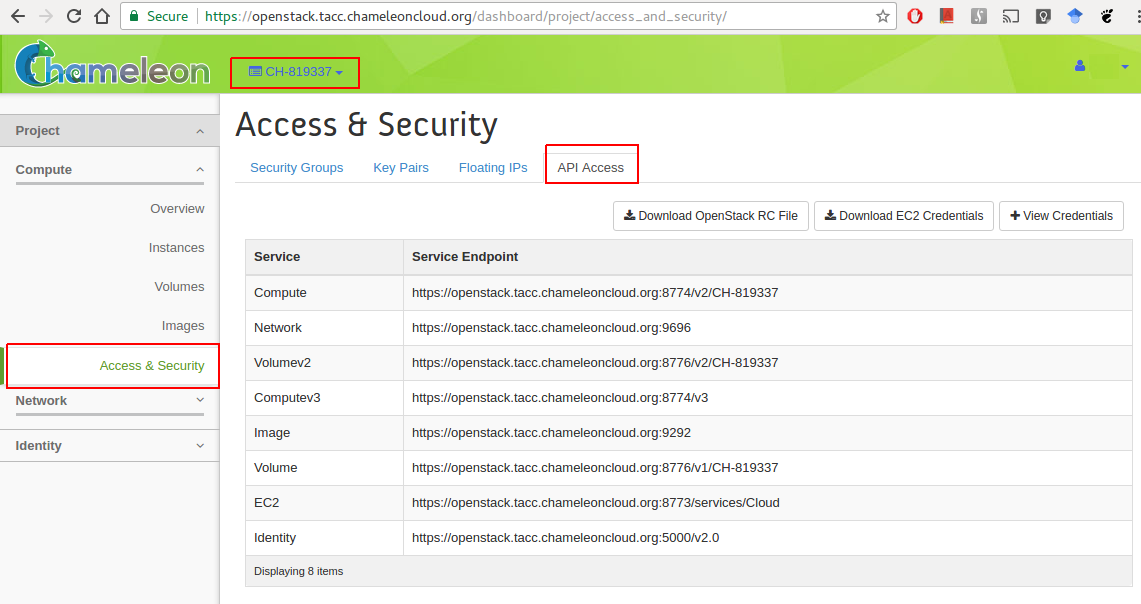
\includegraphics[width=8cm,height=8cm]{section/cloud/chameleon/images/openstack-chameleon-openrc.png}
  \caption{Access and Security GUI}
  \label{F:cc-gui}
\end{figure}


\begin{lstlisting}
mkdir -p ~/.cloudmesh/chameleon
mv ~/Downloads/CH-$CC_PROJECT-openrc.sh ~/.cloudmesh/chameleon/cc-openrc.sh
\end{lstlisting}
%$

Just as in the previous section please add the following to your
openrc.sh file while adapting it appropriately.

\begin{lstlisting}
export CC_PROJECT=CH-819337
export CC_PREFIX=albert-111
\end{lstlisting}

Once you \textit{source} the file, you can use nova command line tools
without sourcing it again.  The environment variables are enabled
while your terminal is alive. IN case you have not stored the original
RC file in the Downloads folder, please copy it from that location
instead.

\subsection{CLI to Manage Virtual Machines}

OpenStack provides a commandline tool called \textit{nova} to manage
virtual machines. To install it please use the command

\begin{lstlisting}
pip install python-openstackclient
\end{lstlisting}

To see if your configuration works and the command is installed, make
sure you have the \verb|cc-openrc.sh| file and sourced it. Than issue
the command

\begin{lstlisting}
$ nova image-list
\end{lstlisting}
%$

You will see an output similar to 

\begin{lstlisting}
+--------------------------------------+------------------+--------+---------+
| ID                                   | Name             | Status | Server  |
+--------------------------------------+------------------+--------+---------+
| be46bd5a-c4a5-4495-ad30-356186d8ff04 | CC-C7-autologin  | ACTIVE |         |
| 1fe5138b-300b-4b30-8d22-e728abbd7773 | CC-CentOS7       | ACTIVE |         |
...
\end{lstlisting}

\subsection{Creating SSH keys}

Naturally you will need an ssh key.  If you do not have an existing
SSH keypair, you can create one. Please see Section~\ref{C:ssh} for
more details:

\begin{lstlisting}
ssh-keygen -t rsa -C mail@example.edu
\end{lstlisting}
%$

\subsection{KeyPair Registration}

Once you have completed the installation of nova, you also need to
register a ssh keypair with openstack to be able to log into the
virtual machines that you start. To register your public key, use:

\begin{lstlisting}
nova keypair-add --pub-key $HOME/ssh/id_rsa.pub $CCPREFIX-key
\end{lstlisting}
%$ 

Once you register your key, you can confirm if your key registration
has been successful by listing the keys:

\begin{lstlisting}
nova keypair-list
\end{lstlisting}

You will see an output similar to:

\begin{lstlisting}
+---------------+-------------------------------------------------+
| Name          | Fingerprint                                     |
+---------------+-------------------------------------------------+
| $CCPREFIX-key | cf:04:06:aa:8b:76:af:77:aa:0a:b5:87:ff:0f:ba:97 |
+---------------+-------------------------------------------------+
\end{lstlisting}
%$


\subsection{Start a new VM instance}

To start new instances you can use the \textit{nova boot} command. It
will start a VM instance. You can use some parameters to specify which
base image and a server size we will use with a name. We use
\textit{CC-Ubuntu16.04} base image in this tutorial which is an
official Ubuntu 16.04 image provided by Chameleon project.

\begin{lstlisting}
nova boot --image CC-Ubuntu16.04 --key-name $CCPREFIX-key --flavor m1.small $CCPREFIX-01
\end{lstlisting}

where the 01 indicates the instance number. Note that we will be
terminating and deleting any VM in our project that does not follow
this naming convention.

\subsection{Floating IP Address}

If your new VM instance is up and running, it needs an external ip
address which is also called floating IP address. A floating IP allows
you to get access to this VM from the internet. Note that chameleon
has a limited number of floating IP addresses and it is best to return
them if not in use. If chameleon runs out of floating IP adresses,
please submit a ticket to chameleon. However in many cases the VM may
only need a an internal IP address as a default. In case you need to
access others, you could even tunnel all connections through a single
floating IP. naturally this would limit data transfers in and out of
chameleon, but is a recommended way to deal with limited floating IPs.

Let us showcase how to associate a floating IP address and access it
via SSH.

\begin{tiny}
\begin{lstlisting}
 nova floating-ip-create ext-net
 +--------------------------------------+----------------+-----------+----------+---------+
 | Id                                   | IP             | Server Id | Fixed IP | Pool    |
 +--------------------------------------+----------------+-----------+----------+---------+
 | 13dc309e-9a82-45af-8a9a-7fbd74f4aec6 | 129.114.111.37 | -         | -        | ext-net |
 +--------------------------------------+----------------+-----------+----------+---------+
\end{lstlisting}
\end{tiny}

Now we have a IP address to assign to a VM instance. In this tutorial,
we will associate \textit{129.114.111.37} to our
albert-111-01 VM instance by:

\begin{lstlisting}
nova floating-ip-associate albert-111-01 129.114.111.37
\end{lstlisting}

Once you completed this step, you are now able to SSH into your VM
instance.  Confirm \textit{ACTIVE} state in your VM to get access.

\begin{tiny}
\begin{lstlisting}
| f19e0ba1-9b76-46f4-896f-378983ab2aa3 | albert-111-01 | ACTIVE  | - | Running  | $CCPROJECT-net=192.168.0.13, 129.114.111.37 |
\end{lstlisting}
\end{tiny}
%$

where 111 is the number from your hid and 01 is the instance number

\begin{lstlisting}
ssh cc@129.114.111.37
\end{lstlisting}

Note that \textit{cc} is login name your VM if you start a VM
with the official Chameleon cloud image.

\subsection{Termination of VM Instance}

If you completed your work on your VM instance, you have to terminate
your VM and release a floating IP address associated with. For
example, we terminate our first instance and the IP address by:

\begin{lstlisting}
nova delete $CCPREFIX-01
nova floating-ip-delete 129.114.111.37
\end{lstlisting}
%$

